\section{Tracking Score}
\subsection{Initialization}
     
    An object being ``out of scene'' actually refers to two scenarios: out of image boundary or too small to be recognized. Without loss of generation, this corresponds to both two cases when objects enter and exit the scene, as an example given in \ref{fig:semantic-entry-exit}. 
    These two cases may be problematic for tracker initialization and termination if not handled correctly. An object may either be initialized when being partially visible or too small to be recognized. 
    Different with the standard object tracking framework, tracking task in real-world use usually relies on external algorithms to find object candidates. Consequently, it is a critical step to the overall performance of any related surveillance task.
    In the following, we show how we apply the scene semantic knowledge into the tracking process and deal with the two scenarios above with a uniform affinity measurement. 

    \begin{figure}
\centering
    \begin{subfigure}{0.4\linewidth}
        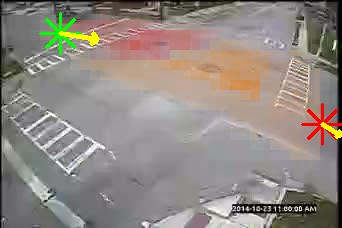
\includegraphics[width=\linewidth]{./img/semantic_tracker/193402-entry-exit-0.jpg}
        \subcaption{}
        \label{subfig:semantic-extry-exit-eg1}
    \end{subfigure}
    \begin{subfigure}{0.4\linewidth}
        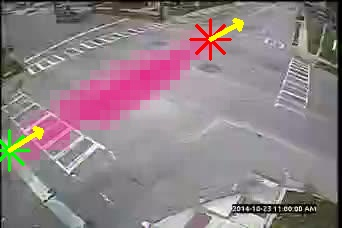
\includegraphics[width=\linewidth]{./img/semantic_tracker/193402-entry-exit-3.jpg}
        \subcaption{}
        \label{subfig:semantic-extry-exit-eg2}
    \end{subfigure}%
    \caption{Two scenarios of object enters and exits: (\subref{subfig:semantic-extry-exit-eg1}): objects enter with a tiny size and move out of image boundary; (\subref{subfig:semantic-extry-exit-eg2}): objects enter from the image boundary and exit with a tiny size in within the frame. Green and red star are the obtained entry/exit hotspots; yellow arrows shows their direction.}
    \label{fig:semantic-entry-exit}
\end{figure}
    
    In computer vision field, for a rigid object, it is widely accepted to use a rectangle as the representation of an object: $\bm{r} = [x, y, w, h]$, where $\bm{p_r}=(x, y)$ is the coordinates of the center point and $(w, h)$ is the width and height.
    A straight line through point $\bm{p}$, parallel to vector $\bm{v}$ is define as $L(\bm{p}, \bm{v})$. Similarly, a ray from point $\bm{p}$ in the direction of vector $\bm{v}$ is define as $R(\bm{p}, \bm{v})$.
    For a rectangle $\bm{r}$ with a center point $\bm{p_r}$, given its moving direction $\bm{v_r}$, we have the following terms for the rectangle, also visually illustrated in Figure \ref{subfig:semantic-box-perp-width} and Figure \ref{subfig:semantic-last-pt}:  
    \begin{itemize}
        \item \emph{Perpendicular width:} the distance between two intersection points of line $L(\bm{p_r}, \bm{v}_{\bm{r}\cdot\text{perp}})$ and the rectangle $\bm{r}$, written as $W(\bm{r}, \bm{v_r})$. 
        \item \emph{Last point:} the intersection point of ray $R(\bm{p_r}, \bm{-v_r})$ with the rectangle $\bm{r}$, written as $P(\bm{r}, \bm{v_r})$.
    \end{itemize}
    Here $\bm{v}_{\bm{r}\text{perp}}$ is the vector perpendicular to $\bm{v_r}$, such that $\bm{v_r}\cdot\bm{v}_{\bm{r}\text{perp}}=0$. Since the object's aspect ratio may vary with the object type and view point of the camera, by defining the \emph{perpendicular width}, both width and height are taken into account. As we will show in the following, the definition of \emph{last point} has a better interpretation of object's moving process, specifically for entering and exiting the scene.

    \begin{figure}
\centering
\begin{subfigure}{0.27\linewidth}
    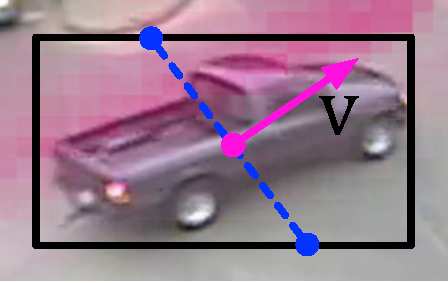
\includegraphics[width=\linewidth]{./img/semantic_tracker/box_perp_width.pdf}
    \subcaption{}
    \label{subfig:semantic-box-perp-width}
\end{subfigure}
\begin{subfigure}{0.27\linewidth}
    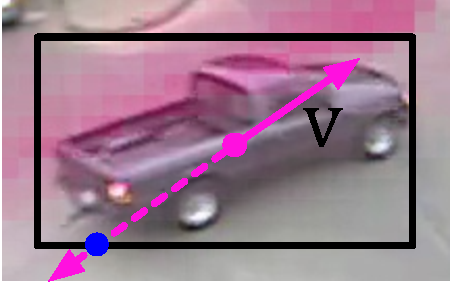
\includegraphics[width=\linewidth]{./img/semantic_tracker/last_pt.pdf}
    \subcaption{}
    \label{subfig:semantic-last-pt}
\end{subfigure}
\begin{subfigure}{0.42\linewidth}
    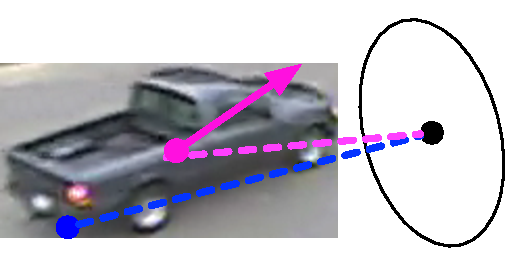
\includegraphics[width=\linewidth]{./img/semantic_tracker/last_pt_dist.pdf}
    \subcaption{}
    \label{subfig:semantic-last-pt-dist}
\end{subfigure}%
\caption{All the solid pink arrows above indicate the moving direction $\bm{v_r}$, the pink dot is the center of the rectangle, blue dots are the intersection points with the rectangle. (\subref{subfig:semantic-box-perp-width}): perpendicular width $W(\bm{r}, \bm{v_r})$ of the object's bounding box wrt. to  direction $\bm{v}_{r}$, shown as the blue dash line. \subref{subfig:semantic-last-pt}: last point $P(\bm{r}, \bm{v_r})$ of the object's bounding box $\bm{r}$, where the dash arrow is $R(\bm{r}, \bm{-v_r})$. (\subref{subfig:semantic-last-pt-dist}): distance between a hotspot with a rectangle's center point and last point $P(\bm{r}, \bm{v_r})$, shown in pink and blue dash lines.}
\label{fig:semantic-perp-width}
\end{figure}

    In real-world applications, with no pre-determined object initialization available, applications usually rely on methods such as background subtraction and object detector, which usually tend to be error-prone.
    With the learned semantic knowledge, we only initialize objects that are around the entry area of the current available topics, with consistent direction and reasonable size. Consequently, noisy candidates with inconsistent motions or far away from the entry area will be effectively eliminated. 
    % \begin{align}
    %     S_\text{dist}(\bm{p}, \bm{p}_1, \bm{p}_2) & = \frac{D\left(\bm{p}, \bm{p}_1\right)}{D\left(\bm{p}_1, \bm{p}_2\right)} \label{eq:entry_dist}\\
    %     S_\text{size}(x_1, x_2) & = 1 - \frac{|x_1 - x_2|}{x_1 + x_2} \label{eq:entry_size}\\
    %     S_\text{direction}(\bm{v}_1, \bm{v}_2) & = \cos(\bm{v}_1, \bm{v}_1) \label{eq:direction}
    % \end{align}

    To quantitatively represent the affinity of an object to a topic $k$'s entry area, we define the following metric:
    \begin{align}
        \begin{split}
        S_\text{entry}(\bm{r}, k) = \frac{1}{3}\times & \Bigl[\Bigl(1-\frac{D(P(\bm{r}, \bm{v_r}), \bm{p}_k(\text{entry}))}{D(\bm{p}_k(\text{entry}), \bm{p}_k(\text{exit}))}\Bigl) \\
        + & \left(1 - \frac{|W(\bm{r}, \bm{v_r}) - W_k(\bm{p_r})|}{W(\bm{r}, \bm{v_r}) + W_k(\bm{p_r})}\right) \\
        + & \cos\big(\bm{v_r}, \bm{v}_k(\text{entry})\big)\Bigl]\label{eq:entry_score}
        \end{split}
    \end{align}
    Here $D(\cdot)$ is the distance measurement of two arbitrary points, we simply use Euclidean distance here. 
    $\bm{p}_k(\text{entry})$ and $\bm{p}_k(\text{exit})$ are the entry and exit point of topic $k$, where the entry/exit points are the Gaussian mean obtained in \S\ref{subsec:hdp-entry-exit}. 
    $W_k(\bm{p_r})$ and $\bm{v}_k(\bm{p_r})$ are the perpendicular width and main direction of topic $k$ at location $\bm{p}_{r}$.
    
    The first term in the square parenthesis is the distance of $P(\bm{r}, \bm{v_r})$ to the exit point, relative to the entry point. It produces a high value for bounding boxes around the entry area, taking the extent of the topic into account without placing any hard threshold. 
    Note that instead of using the center of the rectangle $\bm{p}_{r}$, we use the last point of it. 
    As illustrated in Figure \ref{subfig:semantic-last-pt-dist}, when computing the distance of the object's bounding box and the hotspot, with the moving direction available, considering the last point along the direction measures the movement of the entire object. In other words, despite various object size, by ensuring the last point close to the entry/exit area, the entering/exiting process completes for the entire object.
    The second term will be close to 1 if and only if $W(\bm{r}, \bm{v_r})$ and $W_k(\bm{p_r})$ are similar.
    This penalizes bounding boxes of size either too large or too small, making sure the qualified candidate has a reasonable size relative to the topic's perpendicular width. 


    % Second, as stated in \cite{yanziVehicleTracker}, tracking should start after the object becomes large enough, with more stable and trackable movement. Optical flows are filtered before clustering, therefore, error-prone optical flows do not fall in the entry area extracted on such motion topics.   

    To deal with objects close to the image boundary, we do not initialize a tracker until the last point of the bounding box $\bm{r}$ is apart from the image boundary at least a margin distance; for an object enters with a tiny size, initialization is not considered when the object movement $||\bm{v_r}||_2$ equals $0$, since tiny size usually indicates tiny movement.
    Satisfying the above two cases, we initialize an object with a bounding box $\bm{r}$ once $S_{\text{entry}}(\bm{r}, k) > \sigma_{1}$ for a certain $k$. 

\subsection{Termination}
    When the tracked object manages to reach the exit area, it is quite likely to be well tracked, due to our checking scheme described later in \S\ref{sec:track_eval}. Therefore, we consider terminating a tracker once it is close to its topic's exit area. 
    Similarly, we define a distance measurement of a rectangle $\bm{r}$ with its exit area:
    \begin{align}
        S_\text{exit}(\bm{r}, k) = 1-\frac{D\left(P(\bm{r}, \bm{v_r}), \bm{p}_k(\text{exit})\right)}{D\left(\bm{p}_k(\text{entry}), \bm{p}_k(\text{exit})\right)}
    \end{align}
    where we think the object passes through its exit area when $S_\text{exit}(\bm{r}, k) > \sigma_2$.
    However, in case the object is still able to be correctly tracked, we mark it and keep tracking until it gets lost, we call this phase \emph{extended tracking}. 
    The final trajectory is until the object gets lost. This is especially useful when the object exists with a tiny size. Due to the filtering of the topic model training process, tiny movements are filtered as noises. However, when the object is able to be tracked beyond the exit zone, it is better to keep a longer trajectory. 

\subsection{Tracking Evaluation}
\label{sec:track_eval}
An object's size, location, and motion are well constrained once we have a topic assignment of it. 
Once we initialize a tracker, we check the tracking quality on every frame. In general, we want object move smoothly and follow its visual topic. To quantitatively evaluate this, we define a smoothness term for object's scale change:
\begin{align}
    S(\bm{r}_1, \bm{r}_2) = \frac{1}{2}\left[\left(1-\frac{|w_1- w_2|}{w_1 + w_2}\right) + \left(1-\frac{|h_1 - h_2|}{h_1 + h_2}\right)\right], 
\end{align}
here $w_i$ and $h_i$ are the width and height of rectangle $\bm{r}_{i}$, separately. $S(\bm{r}_1, \bm{r}_2)$ makes sure there is no abrupt scale change between two consecutive frames.
Besides that, to evaluate how well the object is tracked, we have to consider regular tracking and extended tracking differently. 
Before the object reaches its exit area, it is supposed to follow the corresponding visual topic tightly, possibly with occasional stops. So the tracking score is defined as:
\begin{align}
\begin{split}
    S_{\text{track}}(\bm{r}, k, t) = \frac{1}{3}\Bigl[\left(1 - \frac{|W(\bm{r}_t, \bm{v}_{\bm{r}_t}) - W_k(\bm{p}_{\bm{r}_t})|}{W(\bm{r}_t, \bm{v}_{\bm{r}_t}) + W_k(\bm{p}_{\bm{r}_t})}\right) \\
    + S(\bm{r}_t, \bm{r}_{t-1}) + \cos(\bm{v}_{\bm{r}_t}, \bm{v}_k(\bm{p}_{\bm{r}_t}))\Bigl]
\end{split}
\label{eq:track_score}
\end{align}

However, once the object passes through its exit area, it is expected to be truly terminated once it is not well tracked. 
Additionally, zero movements is not allowed. Since the object is not likely to pass through high-density grids in extended tracking phase, we compare the object's moving direction with the exit direction. A similar measurement is defined as:
\begin{align}
    S_{\text{extend}}(\bm{r}, k, t) = \frac{1}{2}\left[S(\bm{r}_t, \bm{r}_{t-1}) + \cos(\bm{v_r}, \bm{v}_k(\text{exit}))\right]\label{eq:track_ext_score}
\end{align}
In both measurement above, the notations are all similar with before, except that a subscript $t$ is added, indicating the corresponding variable at frame $t$. 
$\bm{v}_k(\bm{p}_{\bm{r}_t})$ and $\bm{v}_k(\text{exit})$ are the main direction of topic $k$ at $\bm{r}_{t}$'s center point $\bm{p}_{\bm{r}_t}$, and exit area.
A valid tracking is defined as $S_{\text{track}}(\bm{r}, k, t)>\sigma_{3}$ or $S_{\text{extend}}(\bm{r}, k, t)>\sigma_{4}$, depending on whether it has passed through its exit area. Unqualified tracking will be discarded as failures along the way.
By checking the tracking quality in this way, it is guaranteed that objects manage to pass the exit area follows its topic well and has a smooth movement and scale change. 
Empirically, $\sigma_1\sim\sigma_{4}$ between $0.7\sim0.8$ are a reasonable threshold.
